% Options for packages loaded elsewhere
\PassOptionsToPackage{unicode}{hyperref}
\PassOptionsToPackage{hyphens}{url}
%
\documentclass[
]{article}
\usepackage{amsmath,amssymb}
\usepackage{iftex}
\ifPDFTeX
  \usepackage[T1]{fontenc}
  \usepackage[utf8]{inputenc}
  \usepackage{textcomp} % provide euro and other symbols
\else % if luatex or xetex
  \usepackage{unicode-math} % this also loads fontspec
  \defaultfontfeatures{Scale=MatchLowercase}
  \defaultfontfeatures[\rmfamily]{Ligatures=TeX,Scale=1}
\fi
\usepackage{lmodern}
\ifPDFTeX\else
  % xetex/luatex font selection
\fi
% Use upquote if available, for straight quotes in verbatim environments
\IfFileExists{upquote.sty}{\usepackage{upquote}}{}
\IfFileExists{microtype.sty}{% use microtype if available
  \usepackage[]{microtype}
  \UseMicrotypeSet[protrusion]{basicmath} % disable protrusion for tt fonts
}{}
\makeatletter
\@ifundefined{KOMAClassName}{% if non-KOMA class
  \IfFileExists{parskip.sty}{%
    \usepackage{parskip}
  }{% else
    \setlength{\parindent}{0pt}
    \setlength{\parskip}{6pt plus 2pt minus 1pt}}
}{% if KOMA class
  \KOMAoptions{parskip=half}}
\makeatother
\usepackage{xcolor}
\usepackage{color}
\usepackage{fancyvrb}
\newcommand{\VerbBar}{|}
\newcommand{\VERB}{\Verb[commandchars=\\\{\}]}
\DefineVerbatimEnvironment{Highlighting}{Verbatim}{commandchars=\\\{\}}
% Add ',fontsize=\small' for more characters per line
\newenvironment{Shaded}{}{}
\newcommand{\AlertTok}[1]{\textcolor[rgb]{1.00,0.00,0.00}{\textbf{#1}}}
\newcommand{\AnnotationTok}[1]{\textcolor[rgb]{0.38,0.63,0.69}{\textbf{\textit{#1}}}}
\newcommand{\AttributeTok}[1]{\textcolor[rgb]{0.49,0.56,0.16}{#1}}
\newcommand{\BaseNTok}[1]{\textcolor[rgb]{0.25,0.63,0.44}{#1}}
\newcommand{\BuiltInTok}[1]{\textcolor[rgb]{0.00,0.50,0.00}{#1}}
\newcommand{\CharTok}[1]{\textcolor[rgb]{0.25,0.44,0.63}{#1}}
\newcommand{\CommentTok}[1]{\textcolor[rgb]{0.38,0.63,0.69}{\textit{#1}}}
\newcommand{\CommentVarTok}[1]{\textcolor[rgb]{0.38,0.63,0.69}{\textbf{\textit{#1}}}}
\newcommand{\ConstantTok}[1]{\textcolor[rgb]{0.53,0.00,0.00}{#1}}
\newcommand{\ControlFlowTok}[1]{\textcolor[rgb]{0.00,0.44,0.13}{\textbf{#1}}}
\newcommand{\DataTypeTok}[1]{\textcolor[rgb]{0.56,0.13,0.00}{#1}}
\newcommand{\DecValTok}[1]{\textcolor[rgb]{0.25,0.63,0.44}{#1}}
\newcommand{\DocumentationTok}[1]{\textcolor[rgb]{0.73,0.13,0.13}{\textit{#1}}}
\newcommand{\ErrorTok}[1]{\textcolor[rgb]{1.00,0.00,0.00}{\textbf{#1}}}
\newcommand{\ExtensionTok}[1]{#1}
\newcommand{\FloatTok}[1]{\textcolor[rgb]{0.25,0.63,0.44}{#1}}
\newcommand{\FunctionTok}[1]{\textcolor[rgb]{0.02,0.16,0.49}{#1}}
\newcommand{\ImportTok}[1]{\textcolor[rgb]{0.00,0.50,0.00}{\textbf{#1}}}
\newcommand{\InformationTok}[1]{\textcolor[rgb]{0.38,0.63,0.69}{\textbf{\textit{#1}}}}
\newcommand{\KeywordTok}[1]{\textcolor[rgb]{0.00,0.44,0.13}{\textbf{#1}}}
\newcommand{\NormalTok}[1]{#1}
\newcommand{\OperatorTok}[1]{\textcolor[rgb]{0.40,0.40,0.40}{#1}}
\newcommand{\OtherTok}[1]{\textcolor[rgb]{0.00,0.44,0.13}{#1}}
\newcommand{\PreprocessorTok}[1]{\textcolor[rgb]{0.74,0.48,0.00}{#1}}
\newcommand{\RegionMarkerTok}[1]{#1}
\newcommand{\SpecialCharTok}[1]{\textcolor[rgb]{0.25,0.44,0.63}{#1}}
\newcommand{\SpecialStringTok}[1]{\textcolor[rgb]{0.73,0.40,0.53}{#1}}
\newcommand{\StringTok}[1]{\textcolor[rgb]{0.25,0.44,0.63}{#1}}
\newcommand{\VariableTok}[1]{\textcolor[rgb]{0.10,0.09,0.49}{#1}}
\newcommand{\VerbatimStringTok}[1]{\textcolor[rgb]{0.25,0.44,0.63}{#1}}
\newcommand{\WarningTok}[1]{\textcolor[rgb]{0.38,0.63,0.69}{\textbf{\textit{#1}}}}
\usepackage{longtable,booktabs,array}
\usepackage{calc} % for calculating minipage widths
% Correct order of tables after \paragraph or \subparagraph
\usepackage{etoolbox}
\makeatletter
\patchcmd\longtable{\par}{\if@noskipsec\mbox{}\fi\par}{}{}
\makeatother
% Allow footnotes in longtable head/foot
\IfFileExists{footnotehyper.sty}{\usepackage{footnotehyper}}{\usepackage{footnote}}
\makesavenoteenv{longtable}
\usepackage{graphicx}
\makeatletter
\def\maxwidth{\ifdim\Gin@nat@width>\linewidth\linewidth\else\Gin@nat@width\fi}
\def\maxheight{\ifdim\Gin@nat@height>\textheight\textheight\else\Gin@nat@height\fi}
\makeatother
% Scale images if necessary, so that they will not overflow the page
% margins by default, and it is still possible to overwrite the defaults
% using explicit options in \includegraphics[width, height, ...]{}
\setkeys{Gin}{width=\maxwidth,height=\maxheight,keepaspectratio}
% Set default figure placement to htbp
\makeatletter
\def\fps@figure{htbp}
\makeatother
\setlength{\emergencystretch}{3em} % prevent overfull lines
\providecommand{\tightlist}{%
  \setlength{\itemsep}{0pt}\setlength{\parskip}{0pt}}
\setcounter{secnumdepth}{-\maxdimen} % remove section numbering
\ifLuaTeX
  \usepackage{selnolig}  % disable illegal ligatures
\fi
\usepackage{bookmark}
\IfFileExists{xurl.sty}{\usepackage{xurl}}{} % add URL line breaks if available
\urlstyle{same}
\hypersetup{
  pdftitle={GoalOS: The Proof-of-Evolution Constitution},
  pdfauthor={Vincent Boucher},
  hidelinks,
  pdfcreator={LaTeX via pandoc}}

\title{GoalOS: The Proof-of-Evolution Constitution}
\author{Vincent Boucher}
\date{June 2026}

\begin{document}
\maketitle

\section{GoalOS: The Proof-of-Evolution
Constitution}\label{goalos-the-proof-of-evolution-constitution}

\subsection{AEP-001: The Blockchain-Native Standard for Proof-Carrying
Intelligence
Organizations}\label{aep-001-the-blockchain-native-standard-for-proof-carrying-intelligence-organizations}

\textbf{v12.1 Institutional Presentation Edition}

\textbf{Vincent Boucher}\\
President, QUEBEC.AI \& MONTREAL.AI \textbar{} Sovereign AI, AI-First
Institutions, AI Governance \& Governed Agents\\
June 2026

\begin{quote}
A model can answer. An agent can act. An institution must prove.
\end{quote}

\begin{quote}
Do not put intelligence on-chain. Put proof of intelligence on-chain.
\end{quote}

\begin{quote}
No proof, no evolution. No eval, no propagation. No rollback, no
release.
\end{quote}

\subsection{1. Abstract}\label{abstract}

AI systems should not merely act, remember, or self-improve; they should
produce evidence sufficient to govern what may improve next. This paper
unifies GoalOS, the Agent Evolution Protocol, the Proof Gradient, the
Evolution Ledger, and the Evidence Docket into AEP-001: a
blockchain-native standard for Proof-Carrying Intelligence
Organizations.

The public doctrine is Aim -\textgreater{} Act -\textgreater{} Prove
-\textgreater{} Evolve. The protocol object lifecycle is Commit
-\textgreater{} Execute -\textgreater{} Prove -\textgreater{} Evolve.
GoalOS turns institutional intent into signed, versioned, auditable
commitments. The Run Fabric executes bounded agents off-chain. The Proof
Ledger and Evolution Ledger record proofs, attestations, selection
certificates, rollout receipts, and rollback receipts. The Selection
Gate promotes only what survives evidence, evaluation, risk control,
canary scope, challenge windows, and rollback readiness.

The core claim is architectural and falsifiable: private intelligence
execution should remain off-chain, while public proof commitments,
attestations, reputation, and evolution rights can be coordinated
on-chain. The paper does not claim achieved AGI, ASI, superintelligence,
guaranteed economic return, real-world certification, or
civilization-scale capability. It defines the constitutional doctrine,
protocol objects, evidence standard, benchmarks, threat model, and
commercial deployment path required to test whether agent work can
become governed, reusable, compounding institutional capability.

\begin{itemize}
\tightlist
\item
  A model can answer. An agent can act. An institution must prove.
\item
  Do not put intelligence on-chain. Put proof of intelligence on-chain.
\item
  No proof, no evolution. No eval, no propagation. No rollback, no
  release.
\end{itemize}

\subsection{2. Reader Map}\label{reader-map}

This edition is designed as both a research paper and an institutional
protocol standard. Executives should read the doctrine, commercial
primitive, and deployment model. Engineers should read the object model,
contract suite, schema, and acceptance tests. Governance readers should
read the threat model, claim boundaries, and Evidence Docket standard.

\begin{itemize}
\tightlist
\item
  Executive thesis: why institutions need proof before evolution.
\item
  Constitutional stack: GoalOS, PlanOS, Capability OS, AEP-001, Proof
  Gradient, and Evolution Ledger.
\item
  Protocol standard: object model, schemas, lifecycle, conformance
  levels, and acceptance tests.
\item
  Blockchain boundary: on-chain commitments and attestations; off-chain
  intelligence and private traces.
\item
  Evidence Docket: the institutional proof room for claims, baselines,
  proof packets, costs, risks, and rollback.
\item
  Commercial deployment: proof-backed upgrade rights as the primitive
  product.
\item
  Threat model, claim boundaries, and standards roadmap.
\end{itemize}

\subsection{3. Executive Thesis}\label{executive-thesis}

Frontier models make action cheap; they do not make institutional trust
cheap. The missing layer is not another prompt repository, memory
folder, or ungated swarm. The missing layer is an evidential
constitution: a machine-checkable system that defines what counts as a
valid aim, what counts as execution, what counts as proof, and what
earns the right to influence future behavior.

GoalOS is the constitutional Aim layer. It converts strategic intent
into signed commitments with success criteria, constraints, authority,
risk, budgets, evaluators, and rollback obligations. The Agent Evolution
Protocol is the work standard: it turns commitments into executions,
executions into proof packets, and proof packets into governed evolution
decisions.

The central commercial primitive is the proof-backed upgrade right: the
earned, governed right for an artifact to influence future work after
passing proof, evaluation, scope control, canary rollout, monitoring,
and rollback readiness. This is what makes intelligence reusable without
making unverified claims contagious.

\begin{figure}
\centering
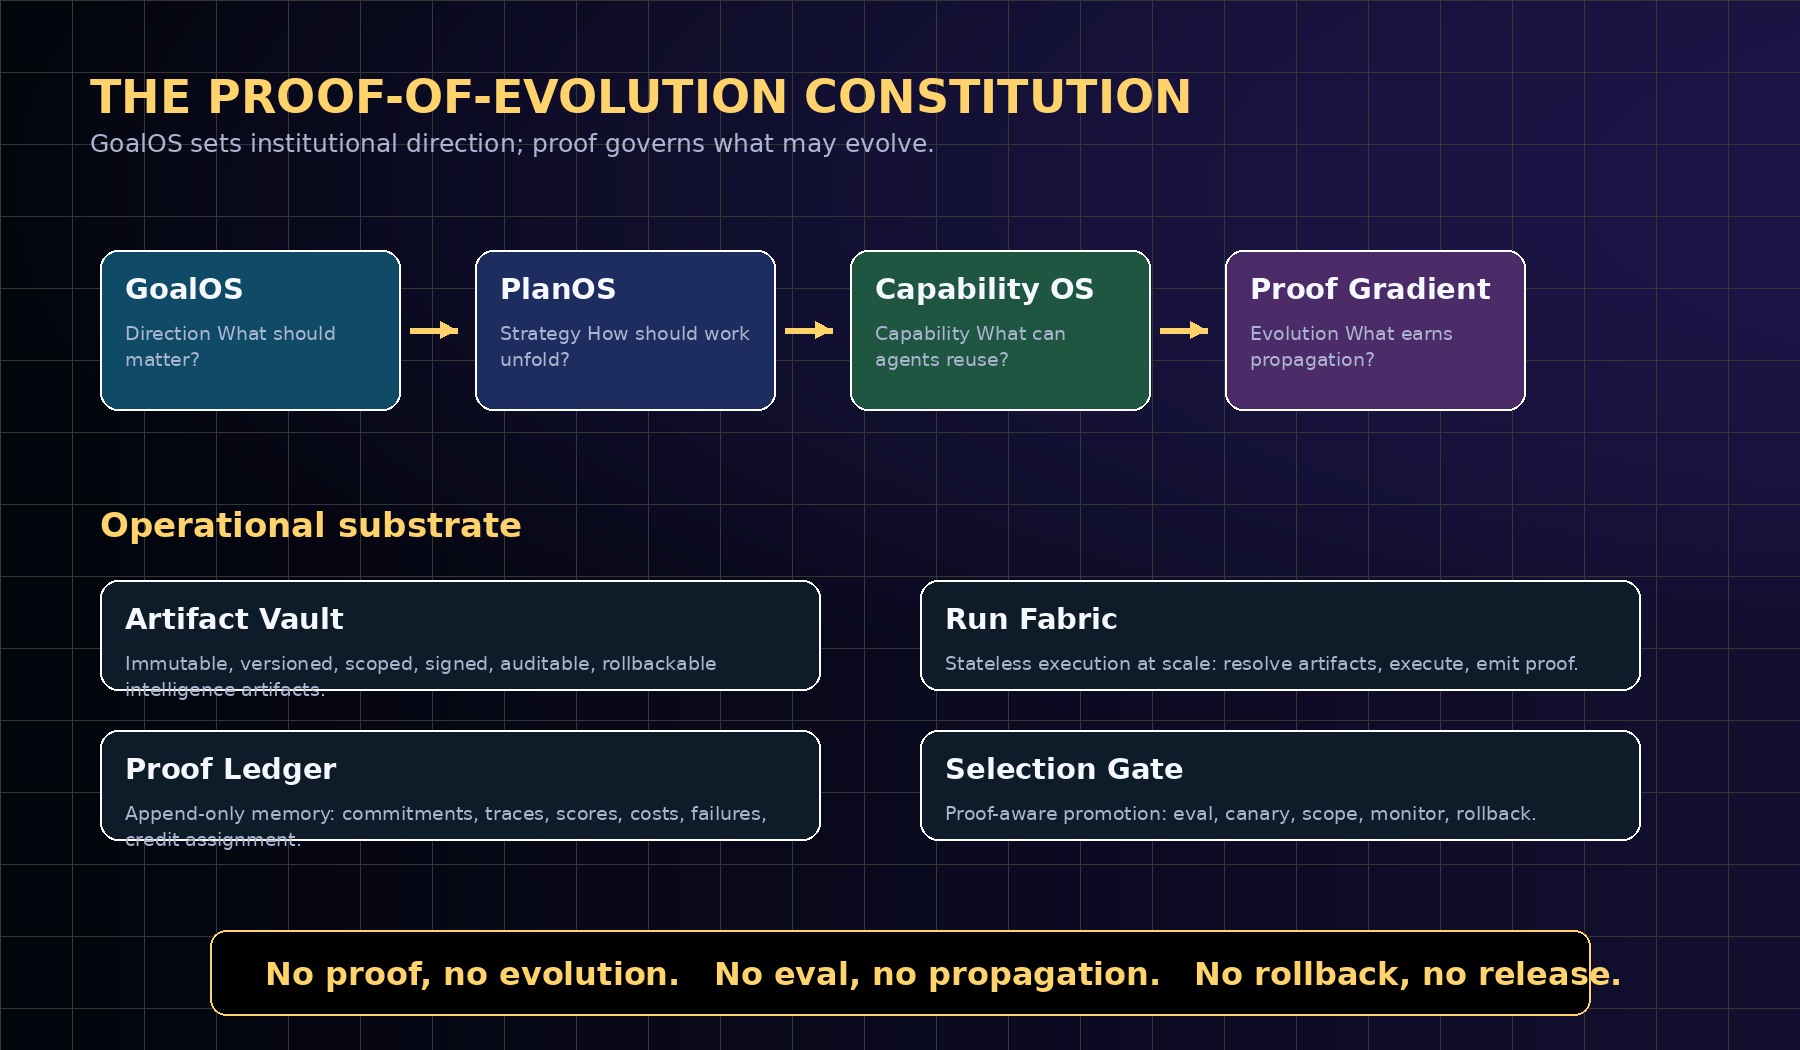
\includegraphics{figures/fig01_constitution_stack.png}
\caption{The unified constitutional stack: GoalOS supplies institutional
direction; AEP-001 defines valid work; the Proof Gradient governs
selection; the operational substrate executes, records, and rolls back.}
\end{figure}

\subsection{4. Canonical Contributions}\label{canonical-contributions}

\begin{longtable}[]{@{}
  >{\raggedright\arraybackslash}p{(\columnwidth - 4\tabcolsep) * \real{0.3333}}
  >{\raggedright\arraybackslash}p{(\columnwidth - 4\tabcolsep) * \real{0.3333}}
  >{\raggedright\arraybackslash}p{(\columnwidth - 4\tabcolsep) * \real{0.3333}}@{}}
\toprule\noalign{}
\begin{minipage}[b]{\linewidth}\raggedright
Contribution
\end{minipage} & \begin{minipage}[b]{\linewidth}\raggedright
What it establishes
\end{minipage} & \begin{minipage}[b]{\linewidth}\raggedright
Why it matters
\end{minipage} \\
\midrule\noalign{}
\endhead
\bottomrule\noalign{}
\endlastfoot
GoalOS as Constitution & A signed Aim layer for institutional goals,
constraints, authority, risk, budget, and evaluators. & Makes
organizational intent auditable before agents act. \\
AEP-001 Standard & A formal object model for GoalOSCommit,
RunCommitment, ProofPacket, EvalAttestation, SelectionCertificate,
RolloutReceipt, RollbackReceipt, Proof-Carrying Artifact, and
EvolutionLedgerEntry. & Makes agent evolution implementable and
testable. \\
Proof Gradient & A selection law requiring proof, evals, risk controls,
canaries, and rollback before propagation. & Separates capability from
authority. \\
Evolution Ledger & An append-only blockchain proof layer for
commitments, hashes, attestations, selection, rollout, rollback,
reputation, rewards, and slashing. & Allows public accountability
without public private-data leakage. \\
Evidence Docket 6.1 & A public-private proof room containing claims,
baselines, manifests, proof packets, evals, costs, risks, and replay
paths. & Turns public proof pages into audit surfaces, not marketing
pages. \\
Commercial Deployment Doctrine & One repeatable workflow -\textgreater{}
GoalOS commitment -\textgreater{} bounded run -\textgreater{} Evidence
Docket -\textgreater{} selected upgrade -\textgreater{} rollbackable
expansion. & Gives institutions a practical adoption path. \\
Falsifiable Benchmark Program & GoalOS-Bench, ProofGradient-Bench,
ArtifactVault-Bench, RunFabric-Bench, SelectionGate-Bench,
EvolutionLedger-Bench, and SovereignPilot-Bench. & Makes the
constitution scientific by specifying how it can fail. \\
\end{longtable}

\subsection{5. The Unified Doctrine}\label{the-unified-doctrine}

The doctrine has two expressions. Publicly, it is Aim -\textgreater{}
Act -\textgreater{} Prove -\textgreater{} Evolve. Internally, it is
Commit -\textgreater{} Execute -\textgreater{} Prove -\textgreater{}
Evolve. These are not competing loops; they are two views of the same
protocol.

Aim is the human and institutional layer. Commit is the protocol object.
Act is the operational layer. Execute is the runtime event. Prove is the
evidential layer. Evolve is the governed propagation layer.

\begin{figure}
\centering
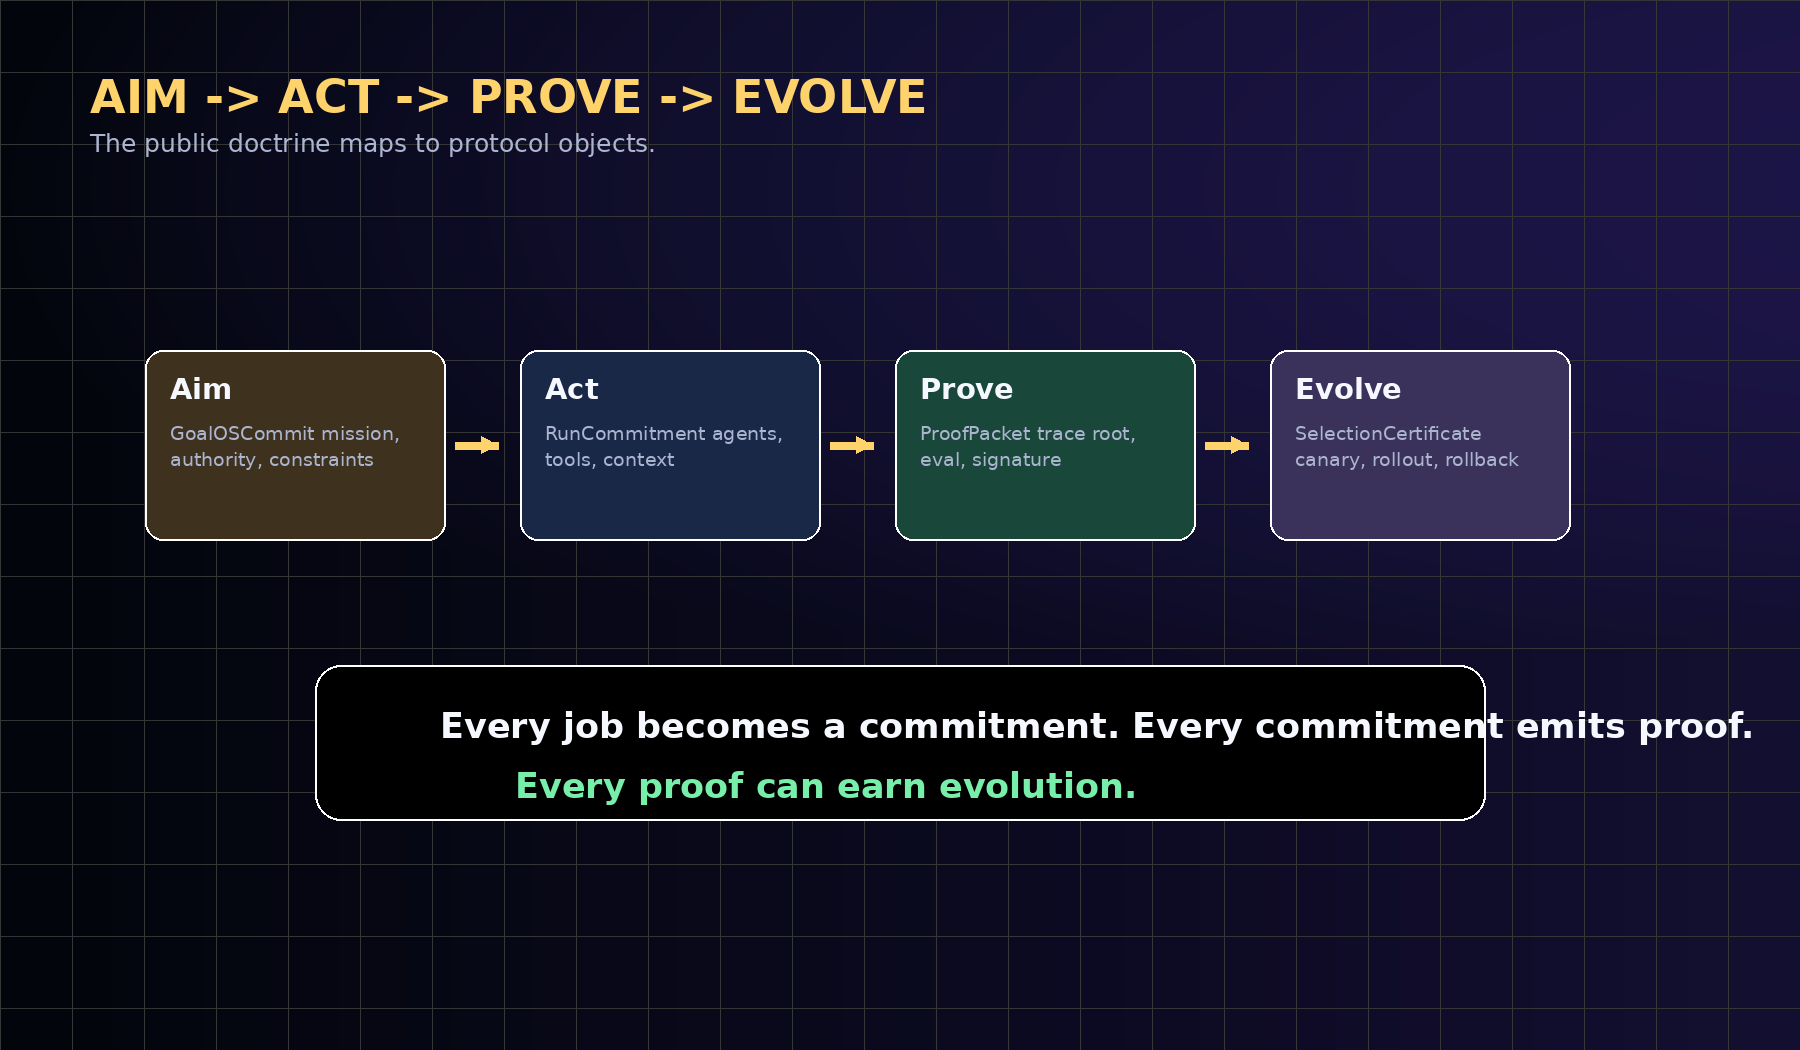
\includegraphics{figures/fig02_loop.png}
\caption{The public doctrine maps to concrete protocol objects. Aim
becomes a commitment; action becomes execution; proof becomes an
attestable packet; evolution becomes a gated certificate.}
\end{figure}

\begin{longtable}[]{@{}
  >{\raggedright\arraybackslash}p{(\columnwidth - 4\tabcolsep) * \real{0.3333}}
  >{\raggedright\arraybackslash}p{(\columnwidth - 4\tabcolsep) * \real{0.3333}}
  >{\raggedright\arraybackslash}p{(\columnwidth - 4\tabcolsep) * \real{0.3333}}@{}}
\toprule\noalign{}
\begin{minipage}[b]{\linewidth}\raggedright
Public doctrine
\end{minipage} & \begin{minipage}[b]{\linewidth}\raggedright
Protocol object
\end{minipage} & \begin{minipage}[b]{\linewidth}\raggedright
Meaning
\end{minipage} \\
\midrule\noalign{}
\endhead
\bottomrule\noalign{}
\endlastfoot
Aim & GoalOSCommit & The institution states the mission, authority,
constraints, success criteria, risk class, budget, evals, and rollback
obligations. \\
Act & RunCommitment & The execution fabric resolves artifacts, agents,
tools, context, policies, credentials, and approval rules. \\
Prove & ProofPacket & The run emits trace roots, output hashes, tool
decisions, policy decisions, eval results, cost, latency, signatures,
and credit assignment. \\
Evolve & SelectionCertificate & The candidate upgrade passes proof
integrity, evaluations, risk thresholds, scope, canary, monitoring, and
rollback readiness. \\
\end{longtable}

\subsection{6. Design Principles}\label{design-principles}

AEP-001 is deliberately small at the core and strict at the boundary. It
scales because execution is stateless, proof is append-only, artifacts
are immutable, learning is asynchronous, improvement is gated,
propagation is scoped, and rollback is mandatory.

\begin{itemize}
\tightlist
\item
  Proof before propagation. No artifact becomes a network-level upgrade
  without evidence.
\item
  Private execution, public commitments. Private prompts, traces,
  customer data, tools, and enterprise documents remain off-chain;
  public commitments remain verifiable.
\item
  Score is advisory; gates are mandatory. A high score cannot bypass
  proof validity, eval pass, scope authorization, rollback readiness, or
  challenge windows.
\item
  Rollback before release. Every promoted upgrade must identify a valid
  rollback target and monitoring condition.
\item
  Artifact-level credit. Credit and blame attach to goals, plans,
  capabilities, tools, policies, evals, context recipes, routing rules,
  and runtime decisions.
\item
  Commercial neutrality. Any model provider, runtime, storage layer,
  evaluator, chain, enterprise, or sovereign institution can implement
  AEP if it respects the proof interfaces.
\item
  Claim discipline. Architecture and strategic horizons are not
  empirical achievements. Claims become empirical only through real
  tasks, baselines, evidence packets, replay, attestations, safety/cost
  ledgers, delayed outcomes, and independent review.
\end{itemize}

\subsection{7. Public-Private Proof
Boundary}\label{public-private-proof-boundary}

The boundary is the central safety and scalability decision. Blockchains
are useful for shared state, deterministic rules, commitments,
settlement, attestations, reputation, and public verification. They are
poor places for private prompts, long traces, raw customer data,
enterprise documents, and expensive inference.

AEP therefore stores the minimum public evidence required to coordinate
trust. Full traces and private execution data stay off-chain. Public
proof is represented through hashes, Merkle roots, signatures,
attestations, and content-addressed pointers.

\begin{figure}
\centering
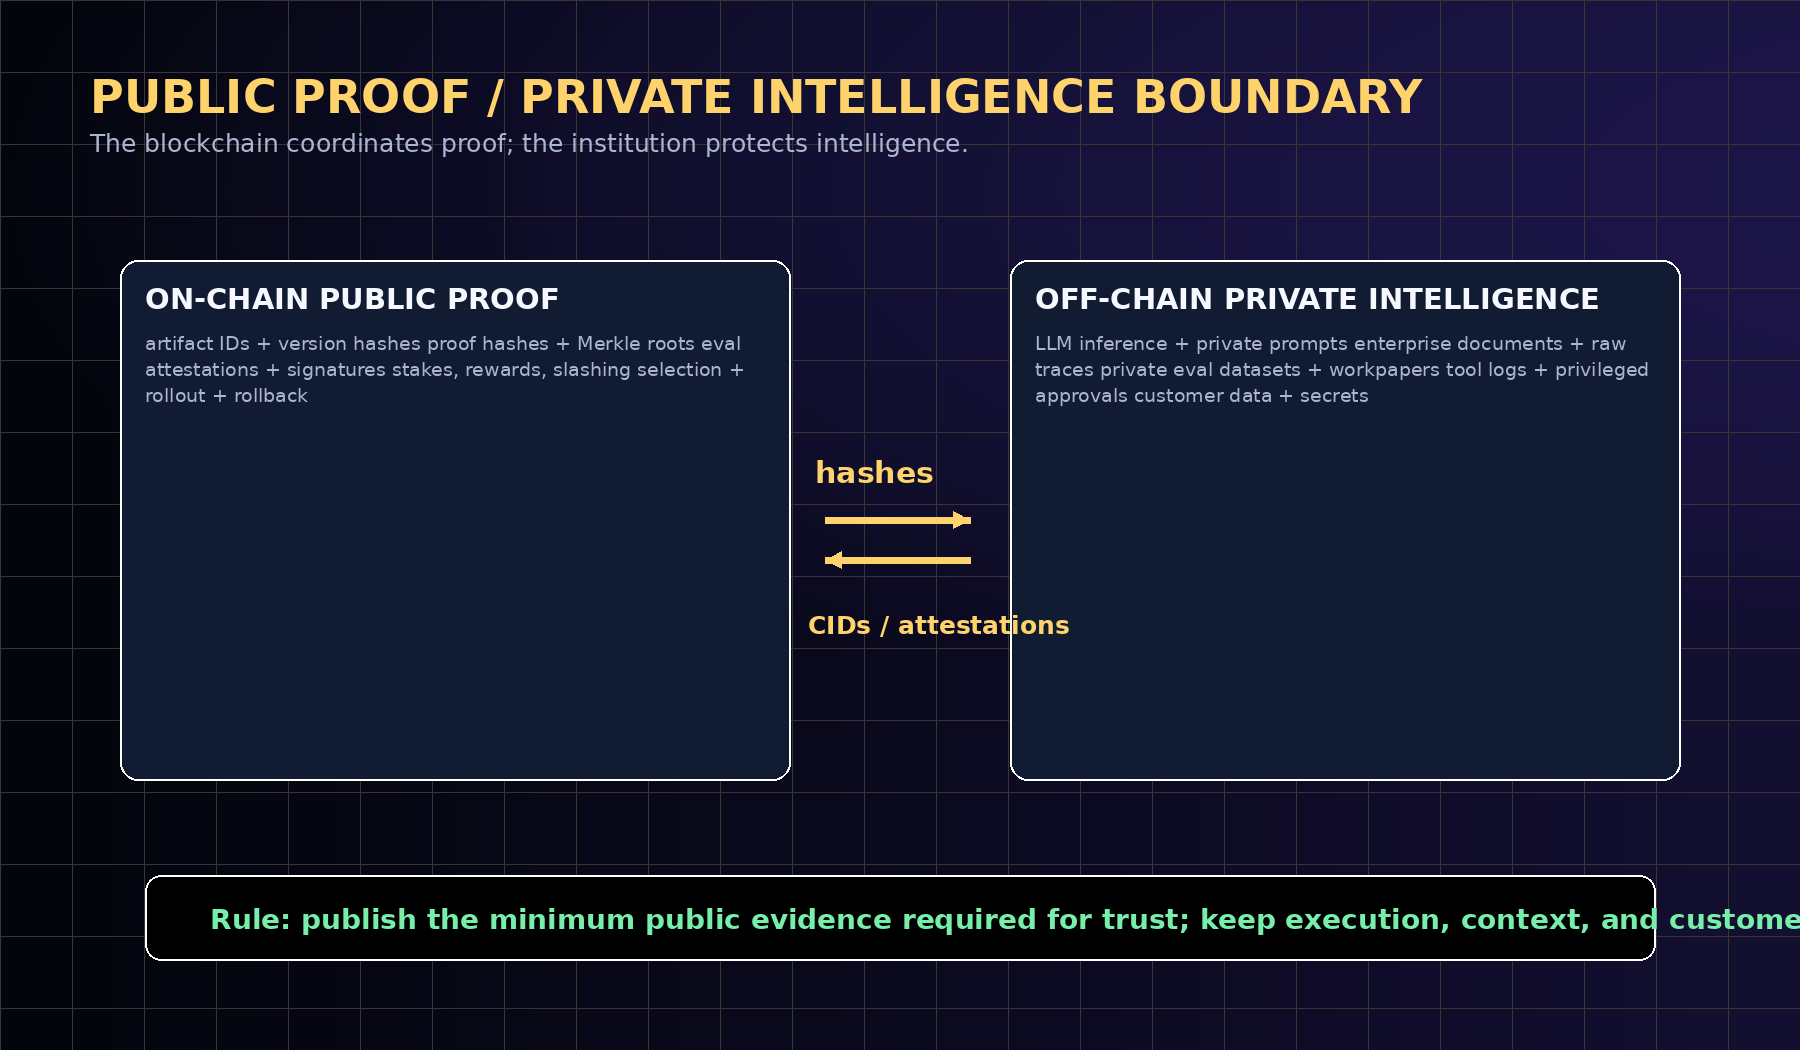
\includegraphics{figures/fig03_boundary.png}
\caption{AEP keeps intelligence execution private and publishes only
proof commitments, content-addressed pointers, attestations, and
selection records.}
\end{figure}

\begin{longtable}[]{@{}
  >{\raggedright\arraybackslash}p{(\columnwidth - 2\tabcolsep) * \real{0.5000}}
  >{\raggedright\arraybackslash}p{(\columnwidth - 2\tabcolsep) * \real{0.5000}}@{}}
\toprule\noalign{}
\begin{minipage}[b]{\linewidth}\raggedright
On-chain public proof
\end{minipage} & \begin{minipage}[b]{\linewidth}\raggedright
Off-chain private intelligence
\end{minipage} \\
\midrule\noalign{}
\endhead
\bottomrule\noalign{}
\endlastfoot
artifact IDs, version hashes, content-addressed pointers & LLM
inference, private prompts, private context, private documents \\
JobCommit hashes, trace roots, output hashes, policy roots & long
traces, raw logs, customer data, sensitive tool outputs \\
EvalAttestations, SelectionCertificates, RolloutReceipts,
RollbackReceipts & private evaluation datasets, privileged approvals,
internal workpapers \\
staking, rewards, slashing events, reputation roots & secret values,
trade secrets, privileged internal rationale \\
public-safe Evidence Docket manifests & private audit appendices
available under scoped review \\
\end{longtable}

\subsection{8. AEP-001 Normative
Vocabulary}\label{aep-001-normative-vocabulary}

AEP-001 uses standards-style keywords for interoperability. MUST means
required for conformance. SHOULD means recommended unless a documented
institutional reason exists. MAY means optional. PUBLIC means safe to
commit, hash, attest, or expose under the protocol. PRIVATE means kept
in controlled storage, disclosed only through scoped audit or verifier
mechanisms where available.

\begin{figure}
\centering
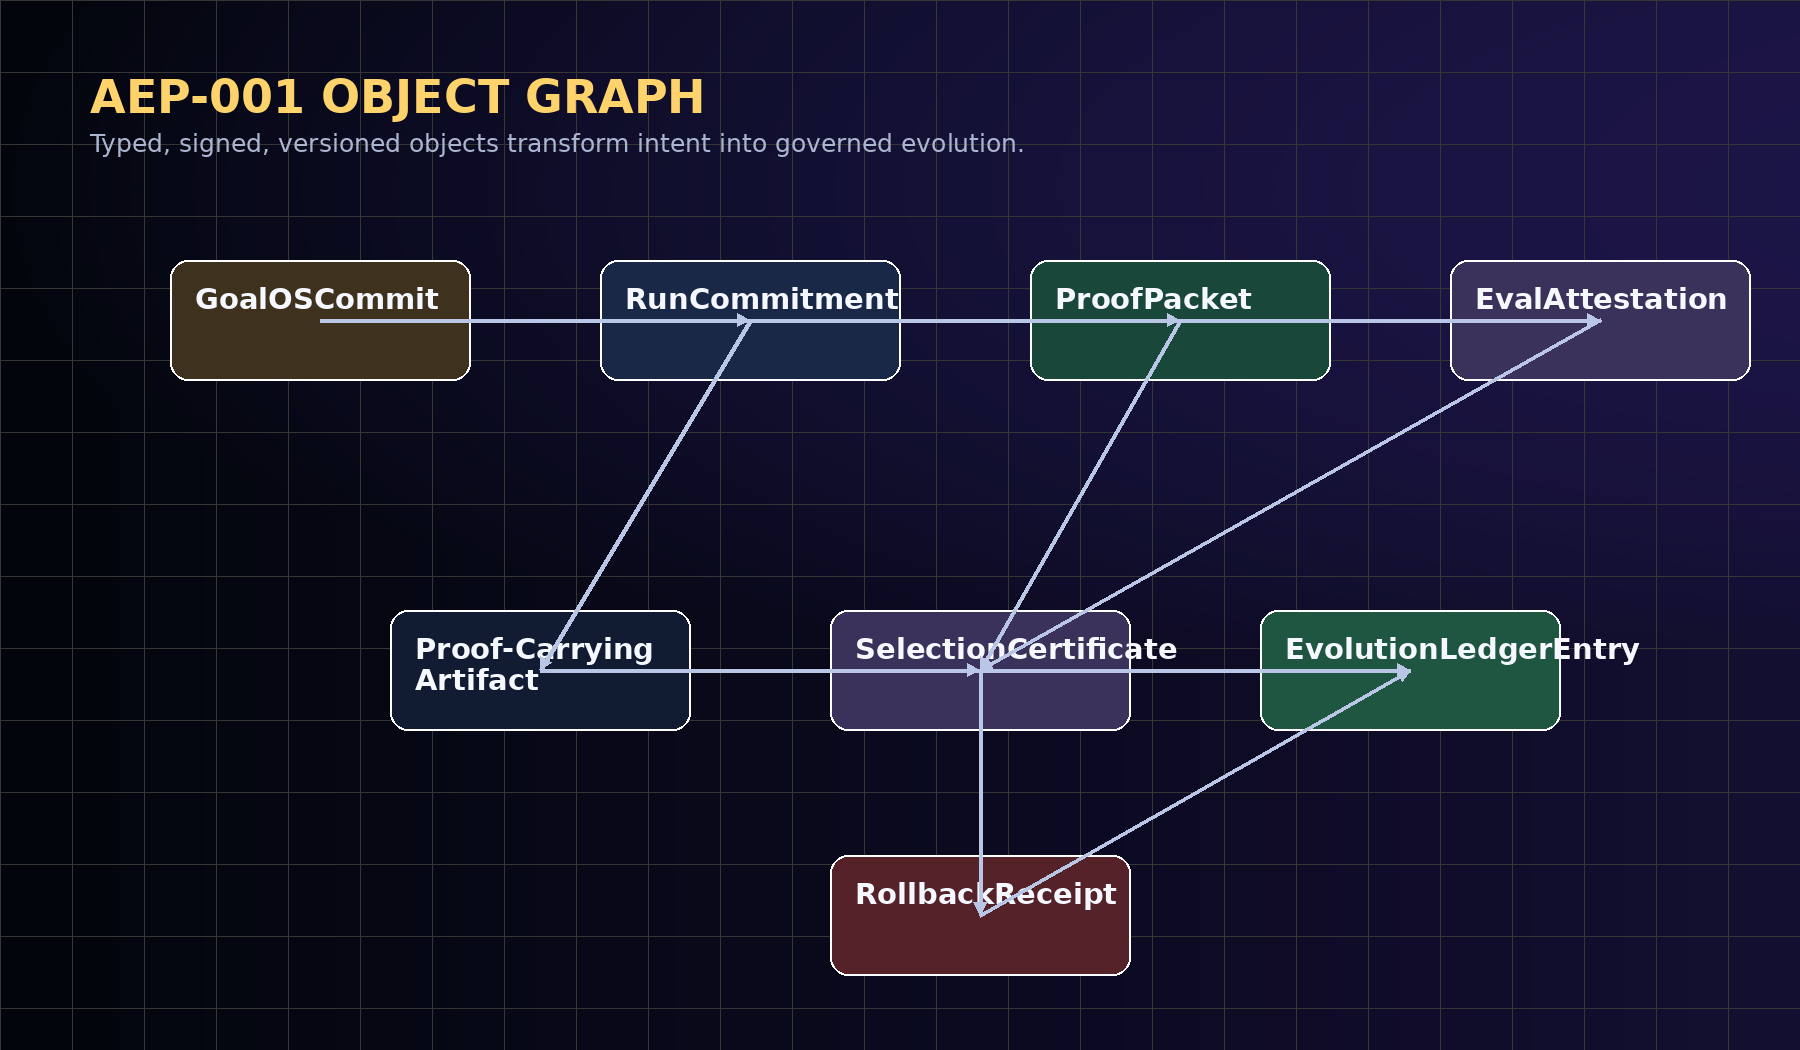
\includegraphics{figures/fig04_object_graph.png}
\caption{AEP-001 object graph. The protocol transforms institutional
intent into proof-carrying evolution through typed, signed, versioned
objects.}
\end{figure}

\begin{longtable}[]{@{}
  >{\raggedright\arraybackslash}p{(\columnwidth - 2\tabcolsep) * \real{0.5000}}
  >{\raggedright\arraybackslash}p{(\columnwidth - 2\tabcolsep) * \real{0.5000}}@{}}
\toprule\noalign{}
\begin{minipage}[b]{\linewidth}\raggedright
Term
\end{minipage} & \begin{minipage}[b]{\linewidth}\raggedright
Definition
\end{minipage} \\
\midrule\noalign{}
\endhead
\bottomrule\noalign{}
\endlastfoot
GoalOSCommit & The signed institutional Aim object: goal, constraints,
authority, risk, budget, evals, allowed tools, and rollback
obligations. \\
RunCommitment & The execution contract: agent set, artifact versions,
tool permissions, context roots, policies, and budget. \\
ProofPacket & The attestable record of execution: trace root, output
hash, evals, policy decisions, cost, latency, signatures, and credit
assignment. \\
Proof-Carrying Artifact & Any goal, plan, capability, tool, policy,
eval, context recipe, router, or workflow with versioned evidence and
rollback metadata. \\
SelectionCertificate & The decision object that admits, rejects,
canaries, promotes, pauses, or rolls back a candidate upgrade. \\
EvolutionLedgerEntry & The append-only public record of commitment,
proof, attestation, selection, rollout, rollback, and reputation
change. \\
Evidence Docket & The institutional proof room tying claims to
baselines, proofs, evals, costs, risks, and public/private
boundaries. \\
\end{longtable}

\subsection{9. Formal Object Model}\label{formal-object-model}

Let an institution maintain an artifact universe A, a job stream J, an
agent set X, a policy set P, an evaluator set E, a private evidence
store V, and a public Evolution Ledger L. A GoalOSCommit is the
authority-bearing object that initializes a protocol run.

\begin{Shaded}
\begin{Highlighting}[]
\NormalTok{GoalOSCommit = (}
\NormalTok{  objective, successCriteria, failureCriteria, constraints,}
\NormalTok{  authority, riskClass, budget, deadline,}
\NormalTok{  allowedTools, requiredEvaluators, approvalRules,}
\NormalTok{  dataBoundary, rollbackObligations, claimBoundary}
\NormalTok{)}

\NormalTok{RunCommitment = (}
\NormalTok{  goalOSCommitHash, agentSet, planGraphHash,}
\NormalTok{  artifactVersionRoots, toolPermissionRoot,}
\NormalTok{  contextRoot, policyRoot, runtimeEnvironment,}
\NormalTok{  budgetLimit, latencyLimit, signerSet}
\NormalTok{)}

\NormalTok{ProofPacket = (}
\NormalTok{  runId, runCommitmentHash, traceRoot, outputHash,}
\NormalTok{  policyDecisionRoot, toolHistoryRoot,}
\NormalTok{  evalResultRoot, cost, latency, errors,}
\NormalTok{  creditAssignment, evidenceURI, signatureBundle}
\NormalTok{)}
\end{Highlighting}
\end{Shaded}

\subsection{10. Proof-Carrying Artifact
Standard}\label{proof-carrying-artifact-standard}

The central object of the system is not an agent and not a model. It is
the Proof-Carrying Artifact: any reusable unit of intelligence whose
right to propagate is backed by evidence. Artifacts can be goals, plans,
capabilities, tools, policies, evals, context recipes, routing rules,
approval rules, or workflows.

Each artifact version is immutable. A new version may be proposed, but
it cannot become active merely because it sounds better. It must carry
proof, be evaluated against a baseline, preserve claim boundaries,
include rollback, and pass the Selection Gate.

\begin{longtable}[]{@{}
  >{\raggedright\arraybackslash}p{(\columnwidth - 4\tabcolsep) * \real{0.3333}}
  >{\raggedright\arraybackslash}p{(\columnwidth - 4\tabcolsep) * \real{0.3333}}
  >{\raggedright\arraybackslash}p{(\columnwidth - 4\tabcolsep) * \real{0.3333}}@{}}
\toprule\noalign{}
\begin{minipage}[b]{\linewidth}\raggedright
Field
\end{minipage} & \begin{minipage}[b]{\linewidth}\raggedright
Meaning
\end{minipage} & \begin{minipage}[b]{\linewidth}\raggedright
Institutional value
\end{minipage} \\
\midrule\noalign{}
\endhead
\bottomrule\noalign{}
\endlastfoot
artifactId & Stable identifier for the artifact family. & Gives reusable
intelligence a durable institutional identity. \\
versionHash & Immutable hash of the released version. & Prevents silent
mutation. \\
artifactClass & Goal, plan, capability, tool, policy, eval, context,
router, workflow. & Makes credit assignment typed and auditable. \\
proofHistory & References to ProofPackets and EvalAttestations. & Shows
why the artifact deserves trust. \\
scope & Tenant, domain, risk class, or rollout scope. & Prevents
uncontrolled propagation. \\
rollbackTarget & Safe prior version or recovery procedure. & Makes
release reversible. \\
selectionStatus & draft, candidate, canary, active, rejected,
rolled\_back, deprecated. & Turns lifecycle into governance. \\
\end{longtable}

\subsection{11. The Proof Gradient Selection
Law}\label{the-proof-gradient-selection-law}

The Proof Gradient is a selection law, not a vibe, not a popularity
contest, and not a marketing score. It is the discipline by which local
agent activity becomes institutional evolution. The score is useful, but
the hard gates are constitutional.

\begin{figure}
\centering
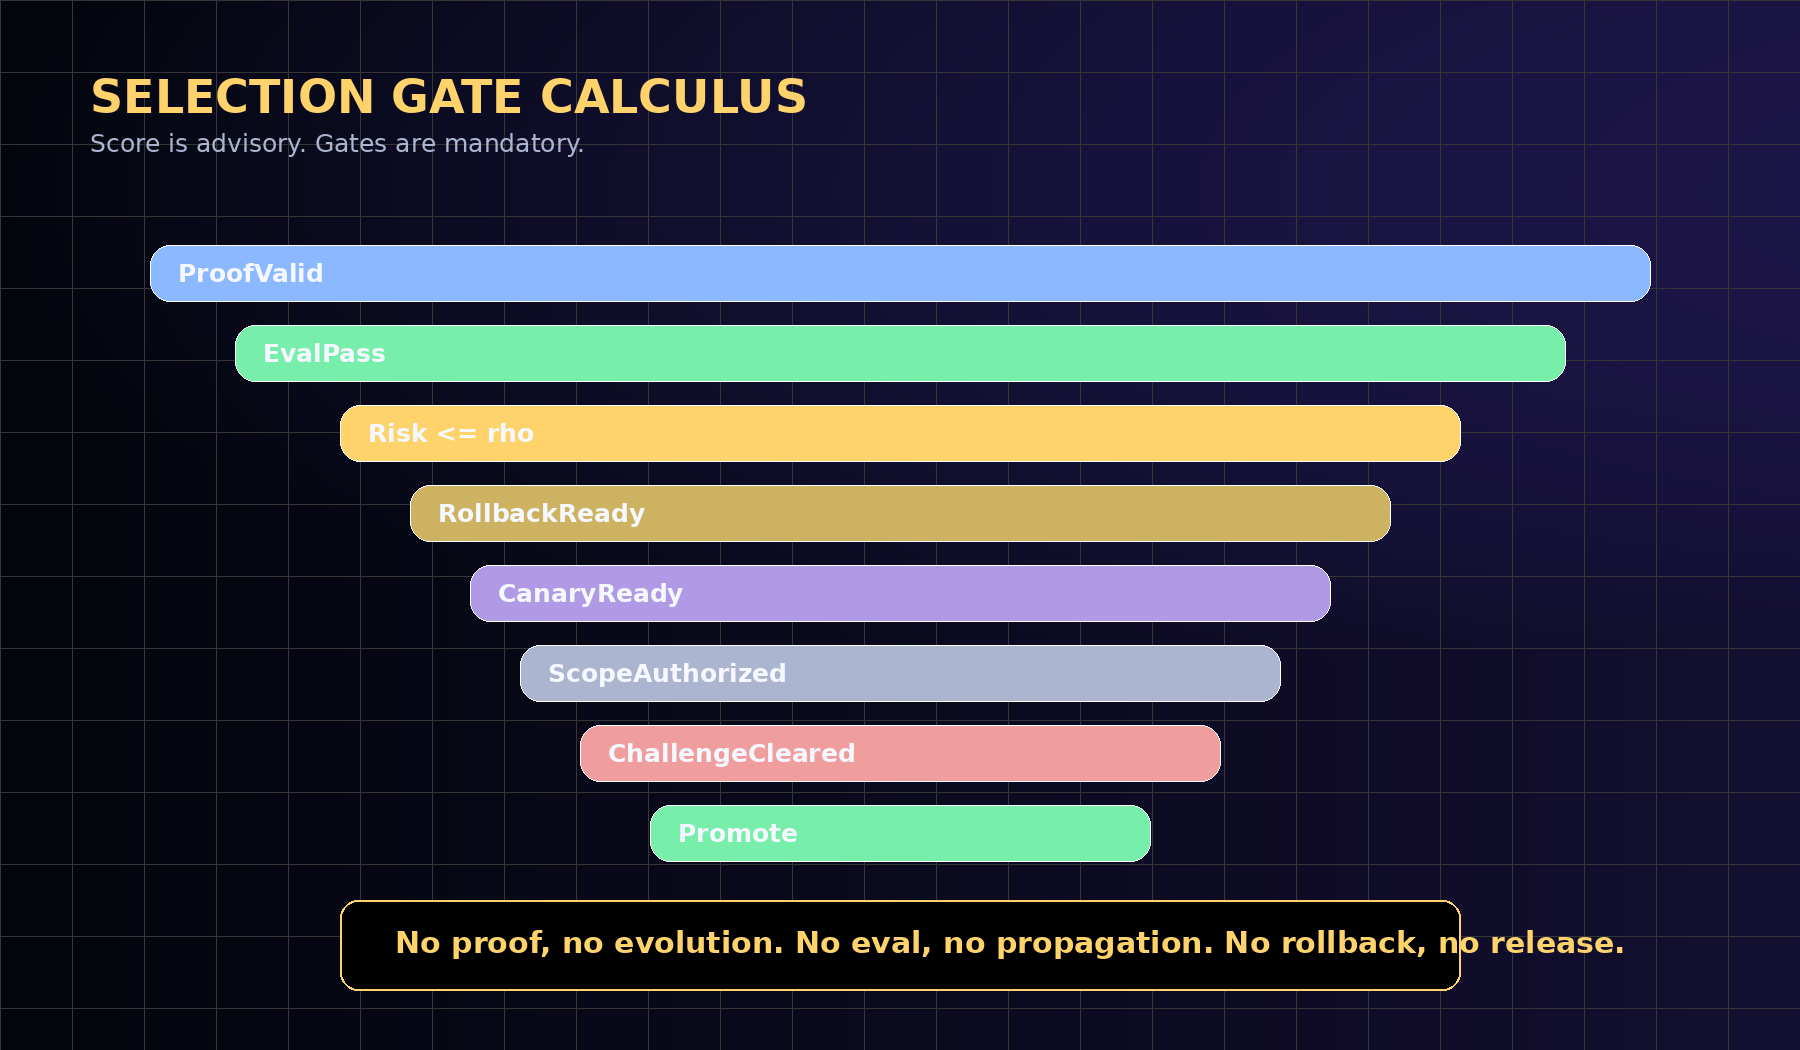
\includegraphics{figures/fig06_selection_gate.png}
\caption{The Selection Gate admits only upgrades whose proof strength,
transfer, and verified value dominate cost, risk, uncertainty, and
rollback debt.}
\end{figure}

\begin{Shaded}
\begin{Highlighting}[]
\NormalTok{PG(U) = wq*QualityDelta(U) + wt*Transfer(U) + wv*VerifiedValue(U)}
\NormalTok{      + wi*EvidenceIntegrity(U)}
\NormalTok{      {-} wc*CostDelta(U) {-} wr*Risk(U) {-} wo*CoordinationOverhead(U)}
\NormalTok{      {-} wb*RollbackDebt(U)}

\NormalTok{Promote(U) iff}
\NormalTok{  ProofValid(U)}
\NormalTok{  AND EvalPass(U)}
\NormalTok{  AND PG(U) \textgreater{}= theta}
\NormalTok{  AND Risk(U) \textless{}= rho}
\NormalTok{  AND RollbackReady(U)}
\NormalTok{  AND CanaryReady(U)}
\NormalTok{  AND ScopeAuthorized(U)}
\NormalTok{  AND ChallengeWindowCleared(U)}
\end{Highlighting}
\end{Shaded}

\subsection{12. Evolution Ledger}\label{evolution-ledger}

The Evolution Ledger is the blockchain-native evidence spine. It does
not store private intelligence. It stores compact commitments,
attestations, decisions, rights, and receipts. Its job is not to know
everything; its job is to make institutional evolution challengeable,
auditable, and difficult to rewrite.

\begin{figure}
\centering
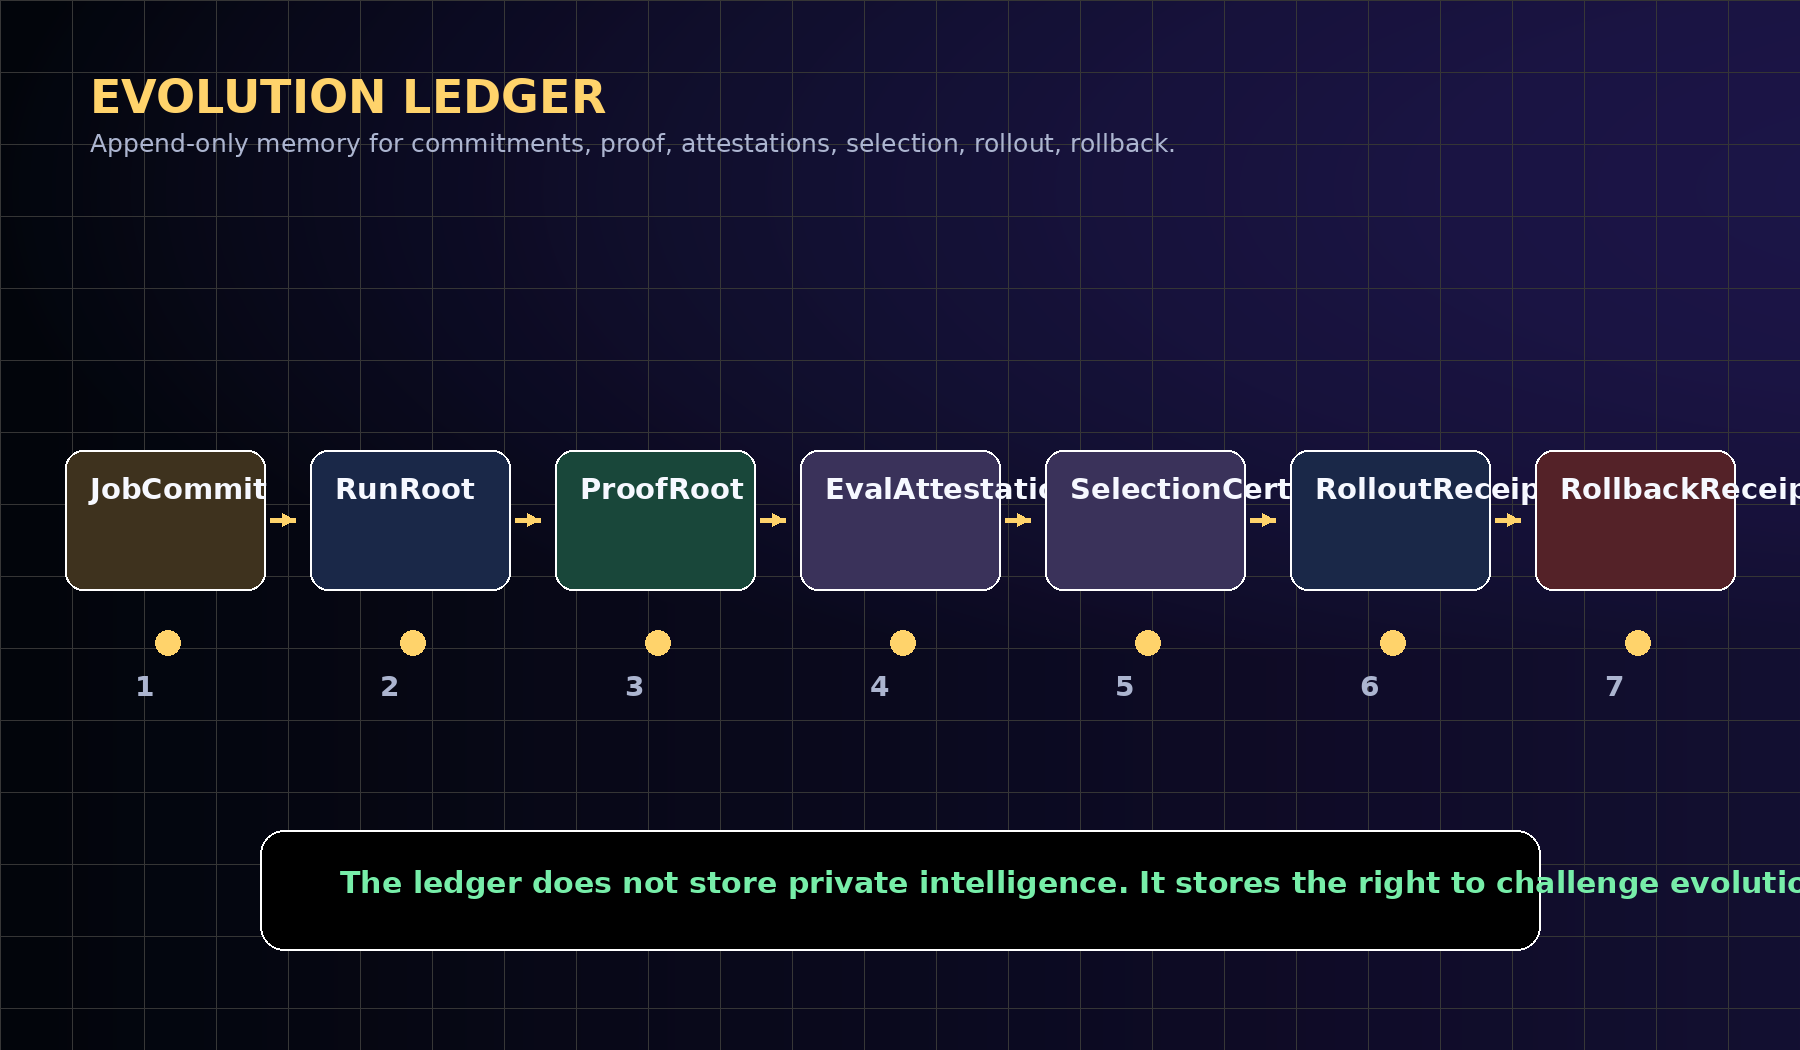
\includegraphics{figures/fig08_evolution_ledger.png}
\caption{Evolution Ledger sequence. The ledger is append-only
institutional memory for proof-carrying evolution.}
\end{figure}

\begin{longtable}[]{@{}
  >{\raggedright\arraybackslash}p{(\columnwidth - 4\tabcolsep) * \real{0.3333}}
  >{\raggedright\arraybackslash}p{(\columnwidth - 4\tabcolsep) * \real{0.3333}}
  >{\raggedright\arraybackslash}p{(\columnwidth - 4\tabcolsep) * \real{0.3333}}@{}}
\toprule\noalign{}
\begin{minipage}[b]{\linewidth}\raggedright
Ledger entry
\end{minipage} & \begin{minipage}[b]{\linewidth}\raggedright
Required public fields
\end{minipage} & \begin{minipage}[b]{\linewidth}\raggedright
Private counterpart
\end{minipage} \\
\midrule\noalign{}
\endhead
\bottomrule\noalign{}
\endlastfoot
JobCommit & commitHash, policyRoot, riskClass, evalRequirements, signer
& full goal context, private documents, privileged constraints \\
RunRoot & runId, artifactRoot, traceRoot, outputHash, executionSigner &
complete trace, raw logs, tool outputs \\
ProofRoot & proofHash, evidenceURI, evalRoot, cost, latency,
signatureBundle & Evidence Docket private appendix \\
EvalAttestation & schemaId, proofRef, baseline, candidate, verdict,
evaluator, signature & raw eval data and evaluator workpapers \\
SelectionCertificate & decision, scope, canary, rollbackTarget,
challengeWindow & internal rationale and approvals \\
RolloutReceipt & percentage, monitoringRoot, safetyThresholds, signer &
tenant-level deployment data \\
RollbackReceipt & rollbackTarget, trigger, status, incidentRoot &
incident details and remediations \\
\end{longtable}

\subsection{13. AEP Contract Suite}\label{aep-contract-suite}

A practical AEP deployment should be modular. The chain should enforce
identities, proofs, attestations, selection, rollout, rollback,
reputation, economics, and governance separation. Execution remains
off-chain; proof rights are coordinated on-chain.

\begin{figure}
\centering
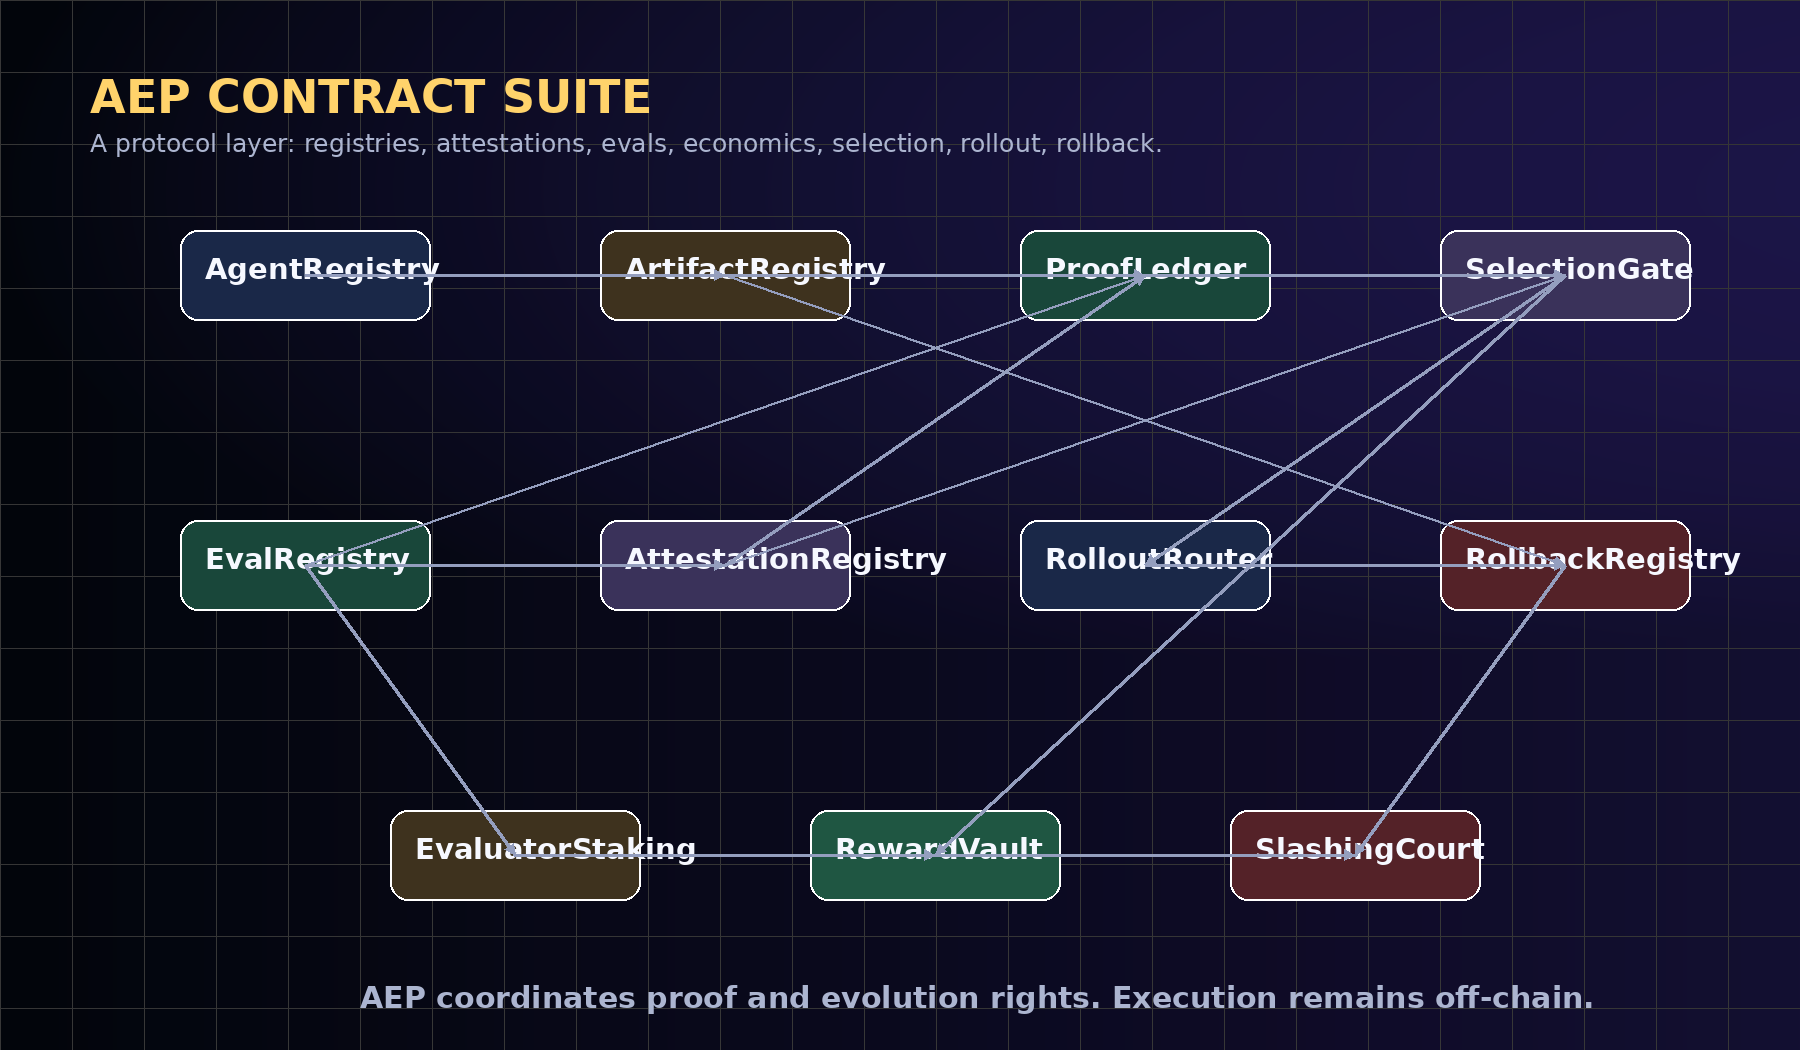
\includegraphics{figures/fig05_contract_suite.png}
\caption{AEP contract modules coordinate registries, attestations,
evaluation, selection, economic settlement, and rollback.}
\end{figure}

\begin{longtable}[]{@{}
  >{\raggedright\arraybackslash}p{(\columnwidth - 2\tabcolsep) * \real{0.5000}}
  >{\raggedright\arraybackslash}p{(\columnwidth - 2\tabcolsep) * \real{0.5000}}@{}}
\toprule\noalign{}
\begin{minipage}[b]{\linewidth}\raggedright
Contract
\end{minipage} & \begin{minipage}[b]{\linewidth}\raggedright
Responsibility
\end{minipage} \\
\midrule\noalign{}
\endhead
\bottomrule\noalign{}
\endlastfoot
AgentRegistry & Registers agent identities, operators, delegated
permissions, credential roots, and reputation roots. \\
ArtifactRegistry & Registers Proof-Carrying Artifacts and immutable
version hashes. \\
RunCommitmentRegistry & Records job/run commitments and public
metadata. \\
ProofLedger & Stores proof roots, evidence pointers, signature bundles,
and public proof metadata. \\
EvalRegistry & Registers evaluator schemas, baseline suites, acceptance
rules, and challenge windows. \\
AttestationRegistry & Records signed claims about runs, evals, policies,
selections, and rollbacks. \\
SelectionGate & Applies hard gates, canary policy, monitoring
thresholds, and rollback requirements. \\
RolloutRouter & Scopes promotions by tenant, domain, risk class, and
rollout percentage. \\
RollbackRegistry & Records rollback targets, triggers, incidents, and
recovery receipts. \\
RewardVault & Settles rewards for evaluated improvement, adoption, and
public-good eval work. \\
SlashingCourt & Handles fraud, false attestations, evaluator collusion,
and challenge resolution. \\
\end{longtable}

\subsection{14. Evidence Docket 6.1}\label{evidence-docket-6.1}

The Evidence Docket is the standard unit of institutional proof. It
separates public proof from private intelligence: sensitive traces,
customer data, prompts, and tool details can remain private, while
commitments, hashes, attestations, scores, and claim boundaries remain
auditable.

A proof page is not a marketing page. It should show artifact evidence,
run evidence, proof ledger evidence, selection evidence, rollback
evidence, security evidence, and claim boundaries. The public viewer
should be able to see what was tested, what passed, what failed, which
baselines were compared, which gates were enforced, and how to rerun or
audit the claim.

\begin{figure}
\centering
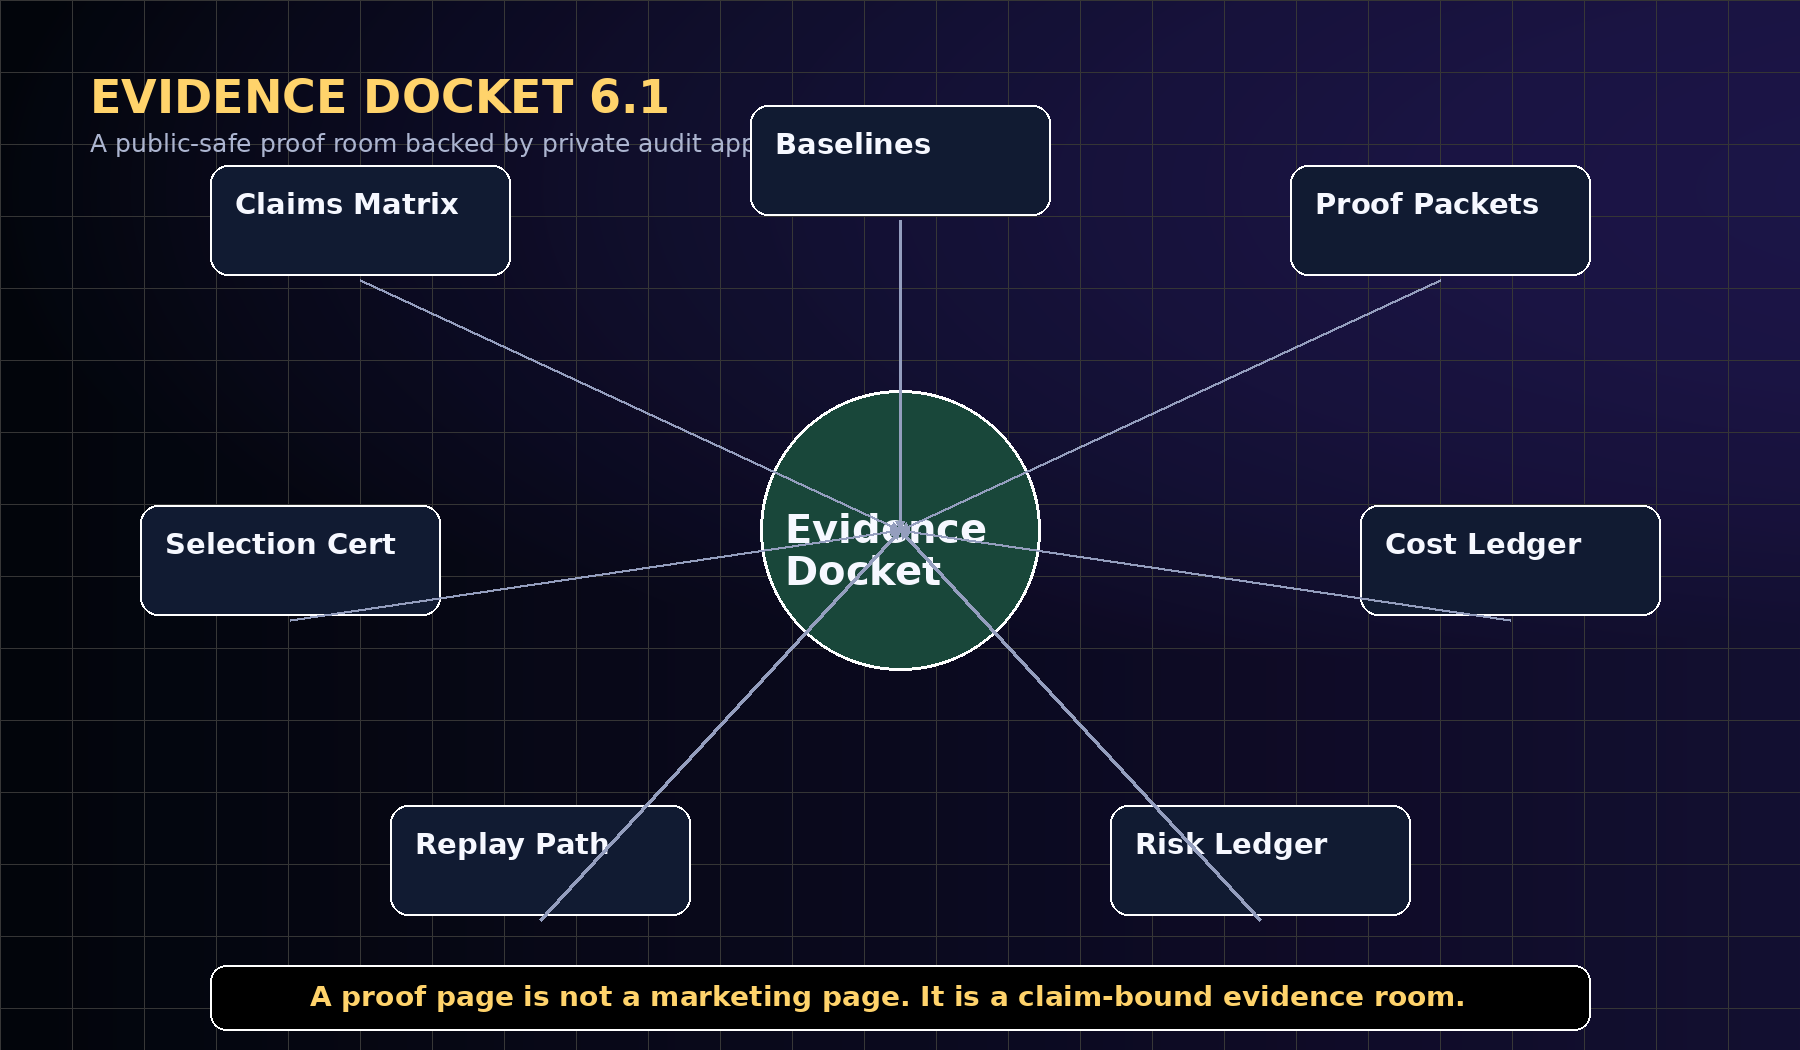
\includegraphics{figures/fig07_evidence_docket.png}
\caption{Evidence Docket 6.1: a public-safe proof room backed by private
audit appendices.}
\end{figure}

\begin{longtable}[]{@{}
  >{\raggedright\arraybackslash}p{(\columnwidth - 2\tabcolsep) * \real{0.5000}}
  >{\raggedright\arraybackslash}p{(\columnwidth - 2\tabcolsep) * \real{0.5000}}@{}}
\toprule\noalign{}
\begin{minipage}[b]{\linewidth}\raggedright
Docket element
\end{minipage} & \begin{minipage}[b]{\linewidth}\raggedright
Purpose
\end{minipage} \\
\midrule\noalign{}
\endhead
\bottomrule\noalign{}
\endlastfoot
Manifest & claim, version, institution, signer, public/private
boundary \\
Claims matrix & what is claimed, not claimed, and required evidence \\
Environment & runtime, model/tool permissions, data boundary, policy
root \\
Baselines & single agent, memory-only, static workflow, unstructured
swarm, incumbent system \\
Proof packets & trace root, output hash, policy decisions, cost,
latency, signatures \\
Evaluator attestations & registered eval schemas, results, challenge
window, auditor notes \\
Selection certificate & promote/reject, scope, canary, rollback target,
monitoring \\
Safety ledger & incidents, blocked actions, unsafe candidates, rollback
drills \\
Public report & non-technical explanation with claim boundary and
reproducibility path \\
Private appendix & privileged traces, workpapers, confidential evaluator
notes under scoped review \\
\end{longtable}

\subsection{15. Flagship Benchmark
Suite}\label{flagship-benchmark-suite}

A constitution becomes scientific only when it can fail. The flagship
benchmark suite evaluates whether evidence-backed evolution works better
than static baselines, memory-only baselines, skill-curation-only
baselines, unstructured swarms, and ungated self-improvement.

\begin{longtable}[]{@{}
  >{\raggedright\arraybackslash}p{(\columnwidth - 4\tabcolsep) * \real{0.3333}}
  >{\raggedright\arraybackslash}p{(\columnwidth - 4\tabcolsep) * \real{0.3333}}
  >{\raggedright\arraybackslash}p{(\columnwidth - 4\tabcolsep) * \real{0.3333}}@{}}
\toprule\noalign{}
\begin{minipage}[b]{\linewidth}\raggedright
Benchmark
\end{minipage} & \begin{minipage}[b]{\linewidth}\raggedright
Tests
\end{minipage} & \begin{minipage}[b]{\linewidth}\raggedright
Primary metrics
\end{minipage} \\
\midrule\noalign{}
\endhead
\bottomrule\noalign{}
\endlastfoot
GoalOS-Bench & Goal specification, revision, auditability, drift
resistance & goal drift rate, policy conflicts, approval trace
completeness \\
ProofGradient-Bench & Prediction of useful upgrades from proof packets &
holdout uplift, false promotion, negative-control rejection \\
ArtifactVault-Bench & Reusable artifact transfer with provenance and
rollback & transfer score, dependency integrity, rollback success \\
RunFabric-Bench & Stateless execution and proof capture at scale &
throughput, cost, trace completeness, failure recovery \\
SelectionGate-Bench & Promotion discipline under adversarial candidates
& unsafe rejection, challenge success, canary precision \\
EvolutionLedger-Bench & Public proof with private intelligence preserved
& redaction safety, audit quality, challengeability, ledger
consistency \\
SovereignPilot-Bench & Institutional deployment without private leakage
& public/private separation, governance audit, user comprehension \\
\end{longtable}

\subsection{16. Commercial Deployment
Doctrine}\label{commercial-deployment-doctrine}

The first commercial deployment should not sell unrestricted autonomy.
It should sell governed improvement: evidence-backed capability adoption
under enterprise and sovereign controls.

The deployment wedge is simple. Choose one repeatable workflow. Convert
it into GoalOS commitments. Execute with bounded agents. Capture proof.
Extract reusable artifacts. Run the Selection Gate. Publish a
public-safe proof room. Keep private intelligence private. Repeat until
the organization can measure whether work is becoming reusable
capability.

Commercial products can include enterprise evidence vaults, proof-backed
procurement records, auditor-ready AI operation rooms, capability
markets, evaluator markets, artifact licensing, agent reputation
profiles, sovereign proof commons, and regulated propagation gates. The
enduring moat is not a demo; it is the evidence graph of what actually
works.

\begin{figure}
\centering
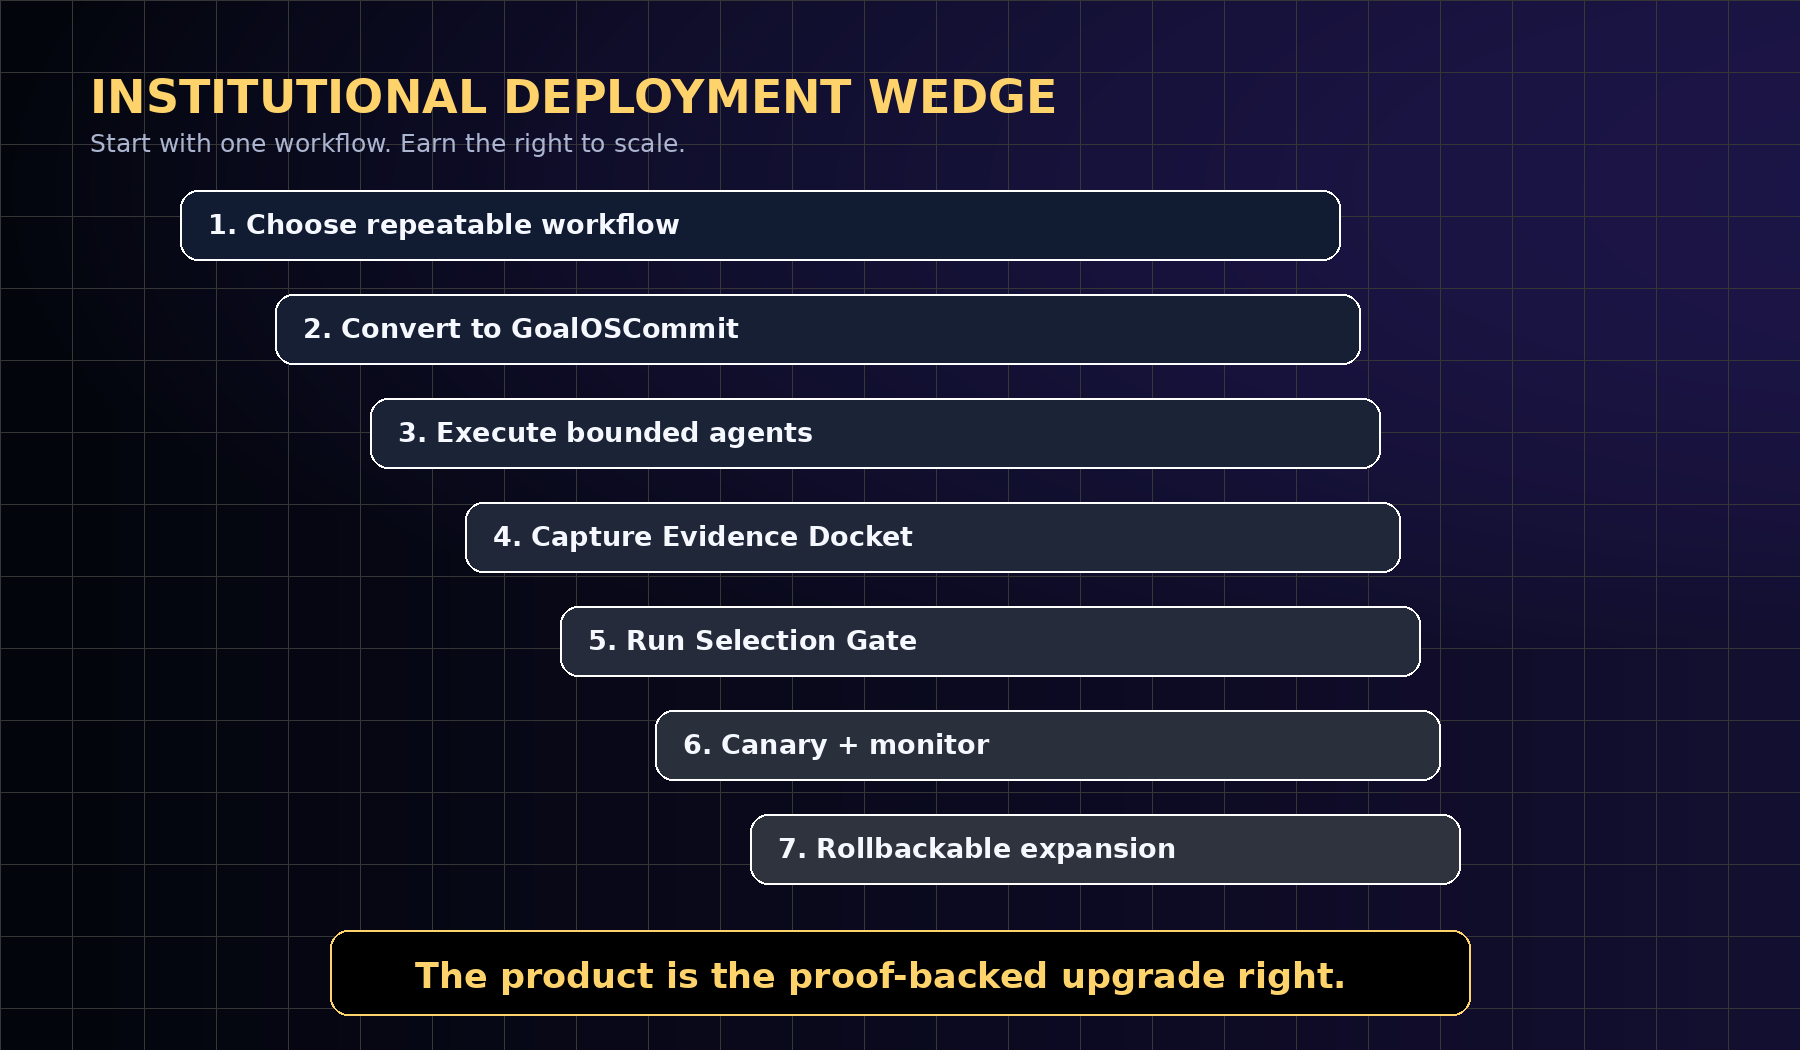
\includegraphics{figures/fig09_deployment.png}
\caption{The institutional deployment wedge: start with one repeatable
workflow and earn the right to scale.}
\end{figure}

\subsection{17. Threat Model}\label{threat-model}

AEP assumes agents, users, evaluators, and operators may be mistaken,
adversarial, collusive, or incentive-misaligned. The protocol therefore
treats proof integrity, privacy, evaluation robustness, and rollback as
first-class security properties.

\begin{longtable}[]{@{}
  >{\raggedright\arraybackslash}p{(\columnwidth - 4\tabcolsep) * \real{0.3333}}
  >{\raggedright\arraybackslash}p{(\columnwidth - 4\tabcolsep) * \real{0.3333}}
  >{\raggedright\arraybackslash}p{(\columnwidth - 4\tabcolsep) * \real{0.3333}}@{}}
\toprule\noalign{}
\begin{minipage}[b]{\linewidth}\raggedright
Threat
\end{minipage} & \begin{minipage}[b]{\linewidth}\raggedright
Failure mode
\end{minipage} & \begin{minipage}[b]{\linewidth}\raggedright
Mitigation
\end{minipage} \\
\midrule\noalign{}
\endhead
\bottomrule\noalign{}
\endlastfoot
False proof & An agent submits forged or incomplete evidence. &
signature verification, trace roots, replay, challenge windows,
evaluator attestations \\
Evaluator collusion & Evaluators approve weak artifacts. & staking,
slashing, diverse evaluators, random audits, independent challenge
markets \\
Reward hacking & Artifacts optimize the score rather than institutional
value. & negative controls, held-out tasks, delayed outcomes, hard
gates, human escalation \\
Privacy leakage & Public proof reveals private prompts, data, or
customer context. & redaction, public/private dockets, content hashes,
scoped audit, data-boundary tests \\
Governance capture & Token votes or insiders bypass evidence. &
governance separation, proof-required execution, challenge rights,
emergency pause \\
Rollback failure & A promoted artifact cannot be safely reverted. &
rollback targets, canary stages, monitoring thresholds, rollback
drills \\
Overclaiming & Strategic scenarios are presented as achieved facts. &
claim-boundary ledger, legal review, empirical evidence thresholds \\
\end{longtable}

\subsection{18. Conformance Levels}\label{conformance-levels}

AEP-001 can be adopted incrementally. The lowest levels validate object
structure; the highest levels support cross-institutional proof,
independent challenge, and governed economic settlement.

\begin{longtable}[]{@{}
  >{\raggedright\arraybackslash}p{(\columnwidth - 4\tabcolsep) * \real{0.3333}}
  >{\raggedright\arraybackslash}p{(\columnwidth - 4\tabcolsep) * \real{0.3333}}
  >{\raggedright\arraybackslash}p{(\columnwidth - 4\tabcolsep) * \real{0.3333}}@{}}
\toprule\noalign{}
\begin{minipage}[b]{\linewidth}\raggedright
Level
\end{minipage} & \begin{minipage}[b]{\linewidth}\raggedright
Name
\end{minipage} & \begin{minipage}[b]{\linewidth}\raggedright
Requirement
\end{minipage} \\
\midrule\noalign{}
\endhead
\bottomrule\noalign{}
\endlastfoot
L0 & Schema-valid & Objects validate against AEP-001 schemas. \\
L1 & Proof-emitting & Runs produce ProofPackets with trace roots, output
hashes, cost, latency, signatures. \\
L2 & Eval-gated & Candidate upgrades require registered evals and
baseline comparisons. \\
L3 & Rollbackable & Every promoted upgrade includes a rollback target
and monitoring conditions. \\
L4 & Attestable & Independent evaluators and auditors can sign
EvalAttestations and SelectionCertificates. \\
L5 & Production-governed & Canary rollout, challenge windows, incident
logs, and governance separation are enforced. \\
L6 & Cross-institutional & Proof-Carrying Artifacts can be adopted
across institutions without exposing private intelligence. \\
\end{longtable}

\subsection{19. Falsification and Acceptance
Tests}\label{falsification-and-acceptance-tests}

The strongest version of this research program is adversarial. It should
publish negative controls, failed upgrades, rejected candidates,
rollback events, and delayed-outcome failures. A system that hides
failure cannot be a proof system.

\begin{longtable}[]{@{}
  >{\raggedright\arraybackslash}p{(\columnwidth - 2\tabcolsep) * \real{0.5000}}
  >{\raggedright\arraybackslash}p{(\columnwidth - 2\tabcolsep) * \real{0.5000}}@{}}
\toprule\noalign{}
\begin{minipage}[b]{\linewidth}\raggedright
Falsification condition
\end{minipage} & \begin{minipage}[b]{\linewidth}\raggedright
Meaning
\end{minipage} \\
\midrule\noalign{}
\endhead
\bottomrule\noalign{}
\endlastfoot
Proof is not predictive & Proof packets fail to identify upgrades that
improve hidden future tasks. \\
Baselines win & Accepted artifacts do not beat strong static, memory,
curation, or swarm baselines under equal budget. \\
Gate is gameable & Candidates exploit proxy metrics or evaluator
weaknesses. \\
Rollback fails & Promoted upgrades cannot be safely reverted or
scoped. \\
Evidence is unreplayable & Dockets cannot be independently inspected,
replayed, or audited. \\
Overhead dominates & Coordination, validation, and governance cost
exceed verified value. \\
Privacy boundary breaks & Public proof leaks private intelligence or
customer data. \\
\end{longtable}

\subsection{20. Claim Boundaries and
Governance}\label{claim-boundaries-and-governance}

This paper does not claim achieved AGI, ASI, superintelligence,
autonomous sovereignty, guaranteed ROI, investment returns, legal
advice, financial advice, medical advice, policy advice, safety
certification, external customer production results, energy abundance,
or Kardashev Type II achievement.

It claims a protocol architecture and a falsifiable research program.
The claim becomes empirical only through real tasks, strong baselines,
proof packets, replay, evaluator attestations, safety ledgers, cost
ledgers, delayed-outcome checks, and independent review.

Civilization-scale language is a strategic horizon, not a present-tense
claim. The measurable near-term claim is governed improvement: verified
work becoming reusable capability under evidence, evaluation, rollout,
and rollback.

\subsection{21. One-Page Constitution}\label{one-page-constitution}

Aim. Act. Prove. Evolve. GoalOS gives the network direction. PlanOS
gives it strategy. Capability OS gives it capability. The Proof Gradient
gives it evolution. The Artifact Vault stores reusable intelligence. The
Run Fabric executes agents at scale. The Proof Ledger records what
happened. The Selection Gate promotes only what proved itself.

Every agent acts once. The network learns forever. A model can answer.
An agent can act. An institution must prove. No proof, no evolution. No
eval, no propagation. No rollback, no release.

\subsection{22. Conclusion}\label{conclusion}

The next frontier is not merely larger models, better agents, or larger
repositories. The next frontier is evidential intelligence: institutions
whose agents may act, but whose improvements must prove themselves
before they propagate.

GoalOS defines what the institution is trying to become. AEP-001 defines
how work becomes proof. The Proof Gradient defines what earns evolution.
The Evolution Ledger makes that evolution verifiable across networks.
The Evidence Docket makes claims auditable. The Selection Gate makes
propagation safe.

The constitutional statement is short enough to remember and strict
enough to implement: Aim. Act. Prove. Evolve. A model can answer. An
agent can act. An institution must prove.

\subsection{References}\label{references}

\begin{itemize}
\tightlist
\item
  Boucher, V. (2026a). AGI ALPHA: A Scalable Substrate for Intelligence
  Organizations. Manuscript draft. Used for organizational-substrate
  lineage, Evidence Docket discipline, proof bundles, replay logs,
  safety/cost ledgers, and governed recursive improvement. Token-related
  material is intentionally excluded.
\item
  Boucher, V. (2026b). GoalOS: The Proof Gradient Constitution.
  Manuscript draft. Used for constitutional doctrine, canonical law,
  proof-backed upgrade rights, benchmark suite, and commercial
  deployment model.
\item
  Ethereum Foundation. (2026). Ethereum smart contracts documentation.
\item
  Solidity Documentation. (2026). Solidity language documentation.
\item
  Ethereum Attestation Service. (2026). Attestation protocol
  documentation.
\item
  IPFS Documentation. (2026). Content addressing and CID documentation.
\item
  Ethereum Improvement Proposal ERC-4337. (2026). Account abstraction
  via EntryPoint contract specification.
\item
  Ethereum Improvement Proposal ERC-6551. (2026). Token-bound accounts
  specification.
\item
  Chainlink Documentation. (2026). Functions and CCIP documentation.
\item
  OpenZeppelin Contracts. (2026). Governor and governance contracts
  documentation.
\item
  W3C. (2025). Verifiable Credentials Data Model v2.0.
\item
  NIST. (2023). Artificial Intelligence Risk Management Framework 1.0.
\item
  NIST. (2024). Artificial Intelligence Risk Management Framework:
  Generative AI Profile.
\item
  OWASP. (2026). Agentic AI threat modeling and securing agentic
  applications guidance.
\item
  Necula, G. C. (1997). Proof-carrying code. Proceedings of POPL.
\end{itemize}

\end{document}
